\documentclass{121Temp}

\usepackage{amsmath}
\usepackage{amssymb}
\usepackage{amsthm}
\usepackage{commath}
\usepackage{listings}
\usepackage{mathtools}
\usepackage{float}

\usepackage{hyperref}

\usepackage{graphicx}
\graphicspath{ {images/} }

\hwauthor{Jonathan Levine}{jonlevi@sas.upenn.edu}
\hwcourse{BIBB 585}
\hwrecitation{401}
\hwno{5}

% \date{}  % uncomment this line to suppress the current date in the title
% \date{Due: Never}  % or uncomment this line to manually add a date
% \hwonelateday                   % uncomment either this line or the next to
% \hwtwolatedays                  % indicate that you are using an extension

\begin{document}
\maketitle

% Problem 1
\hwproblem
\label{Qa}
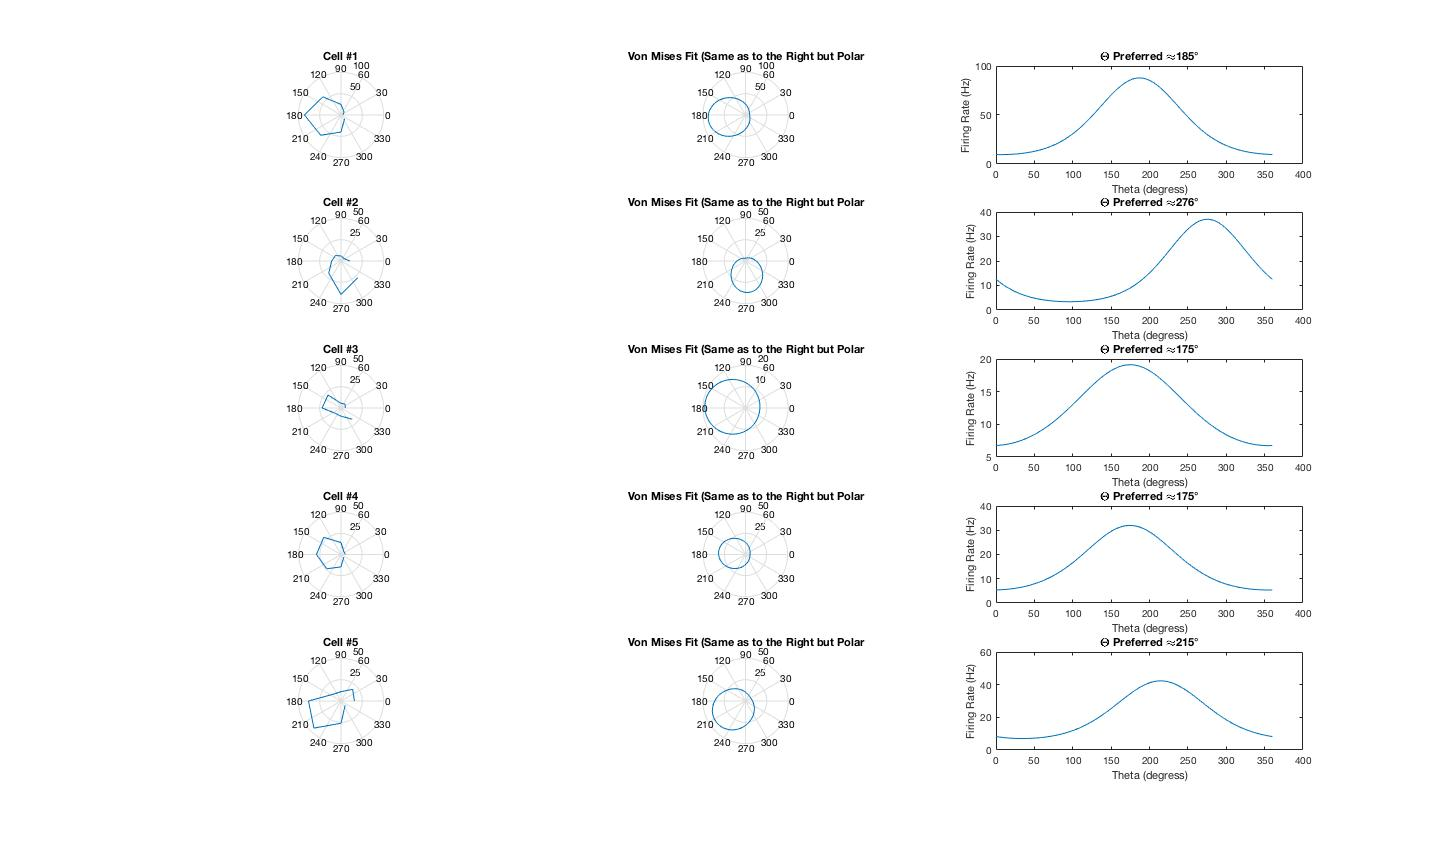
\includegraphics[scale=.35]{part1.jpg}


% Problem 2
\hwproblem

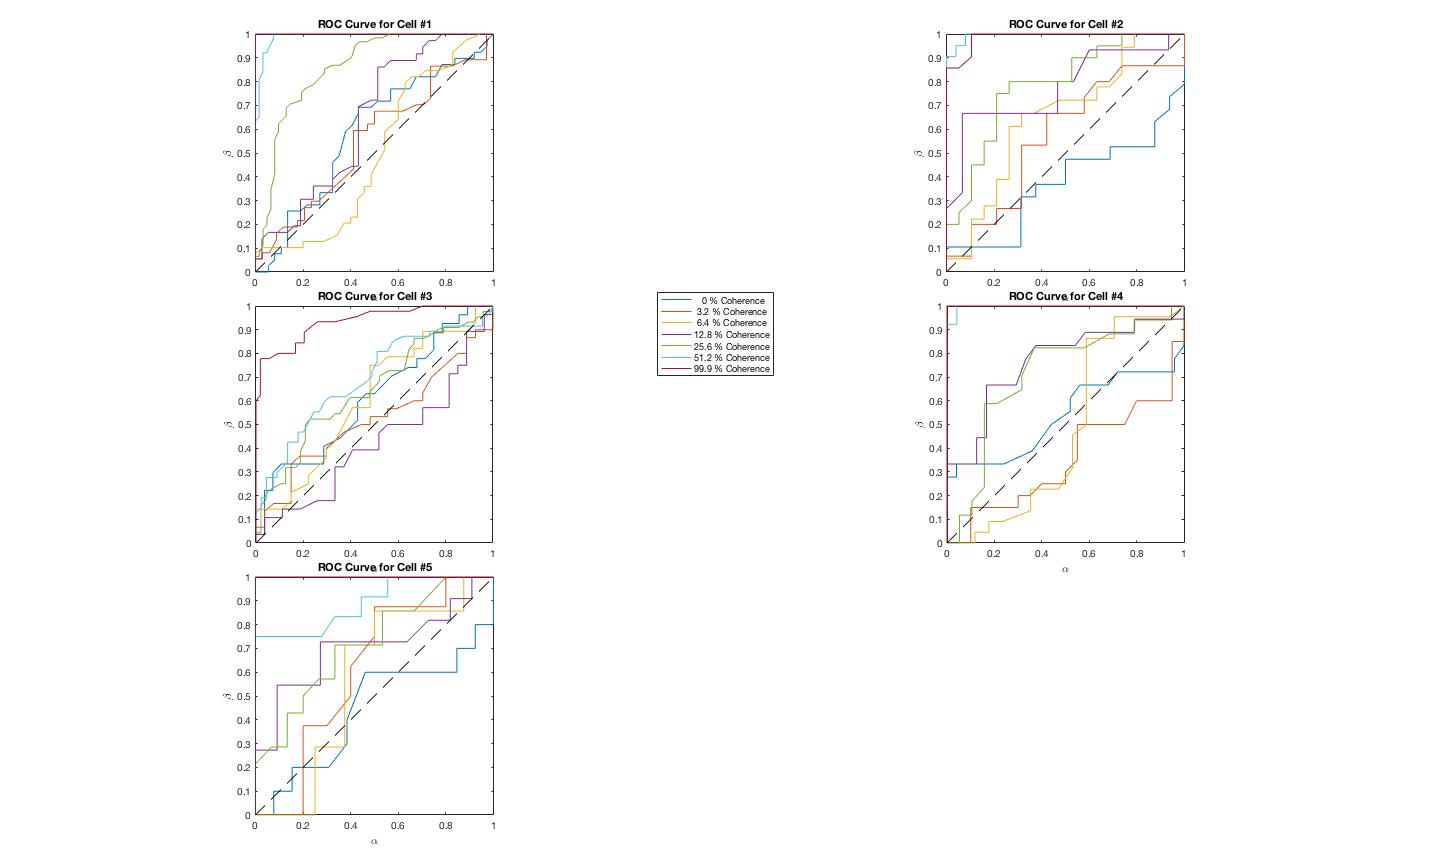
\includegraphics[scale=.40]{roc_curves}


\begin{table}[H]
\centering
\caption{Areas Under the ROC Curves}
\label{my-label}
\begin{tabular}{|l|l|l|l|l|l|l|l|}
\hline
      & 0\%   & 3.2\% & 6.4\% & 12.8\% & 25.6\% & 51.2\% & 99.9\% \\ \hline
Cell1 & 0.587 & 0.551 & 0.495 & 0.642  & 0.859  & 0.990  & 1      \\ \hline
Cell2 & 0.375 & 0.572 & 0.651 & 0.776  & 0.786  & 0.994  & 0.986  \\ \hline
Cell3 & 0.610 & 0.523 & 0.605 & 0.425  & 0.645  & 0.690  & 0.935  \\ \hline
Cell4 & 0.538 & 0.353 & 0.476 & 0.764  & 0.711  & 0.997  & 1      \\ \hline
Cell5 & 0.442 & 0.613 & 0.571 & 0.707  & 0.719  & 0.891  & 1      \\ \hline
\end{tabular}
\end{table}



% Problem 3
\hwproblem
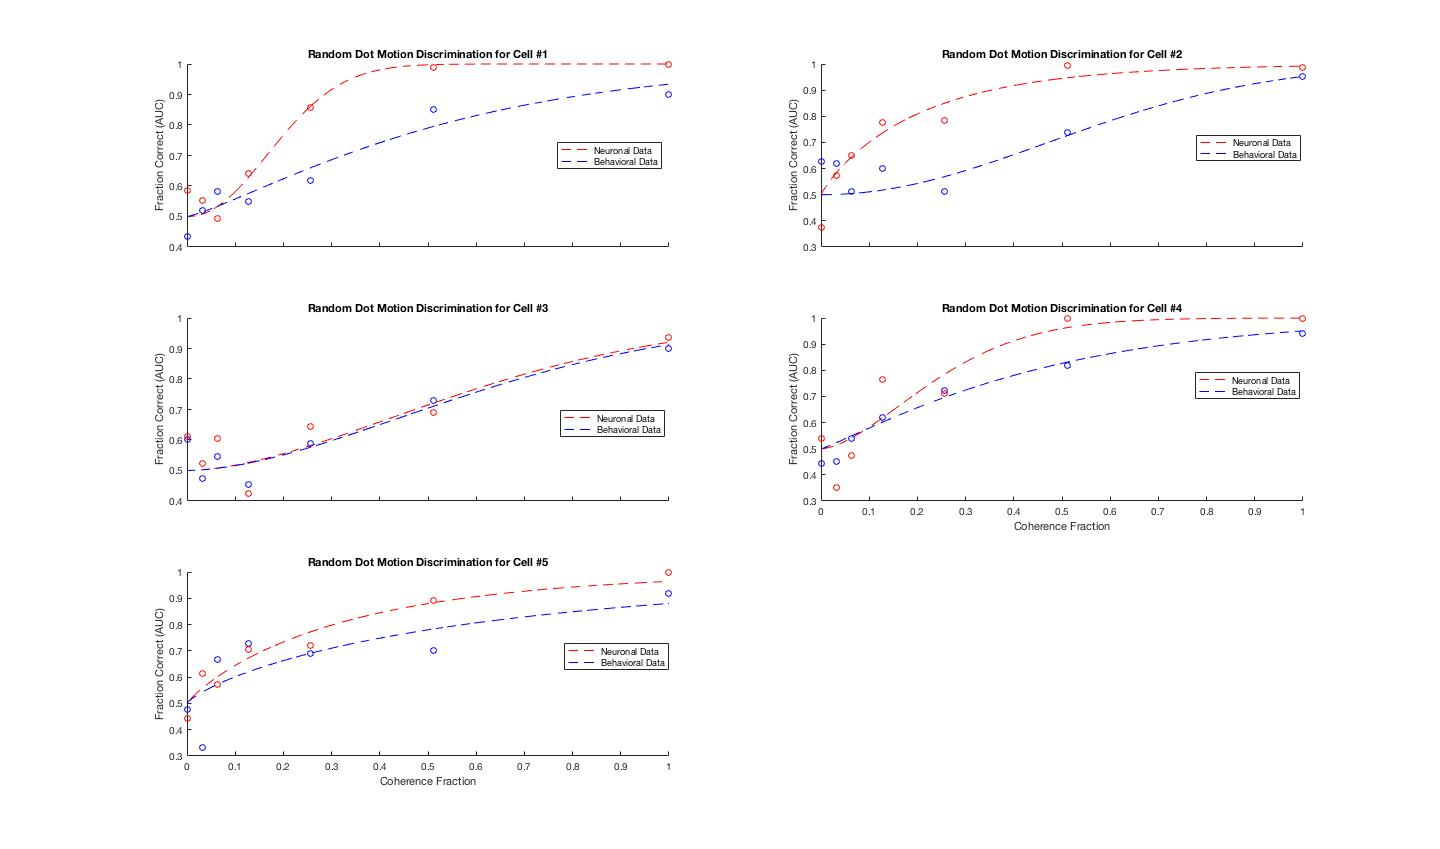
\includegraphics[scale=.70]{metric_curves}




\end{document}